\chapter{Methodology}\label{chapter:methodology}

This chapter presents the methodology for enhancing intraoperative registration using Neural Radiance Fields (NeRFs). First, it provides an overview of the NeRF-based registration approach, followed by details on the implementation framework, optimization procedure, and an examination of various loss functions.

\section{Overview of the NeRF-based Registration Approach}

The core methodology of this thesis builds upon the inverse Neural Radiance Field (iNeRF) approach originally proposed by \textcite{yen2020inerf} and extended for cross-modal intraoperative registration by \textcite{fehrentz2024intraoperative}. Figure~\ref{fig:overview} provides a high-level overview of the approach.

% Placeholder for overview figure

\vspace{1cm}
\begin{figure}[htbp]
  \centering
  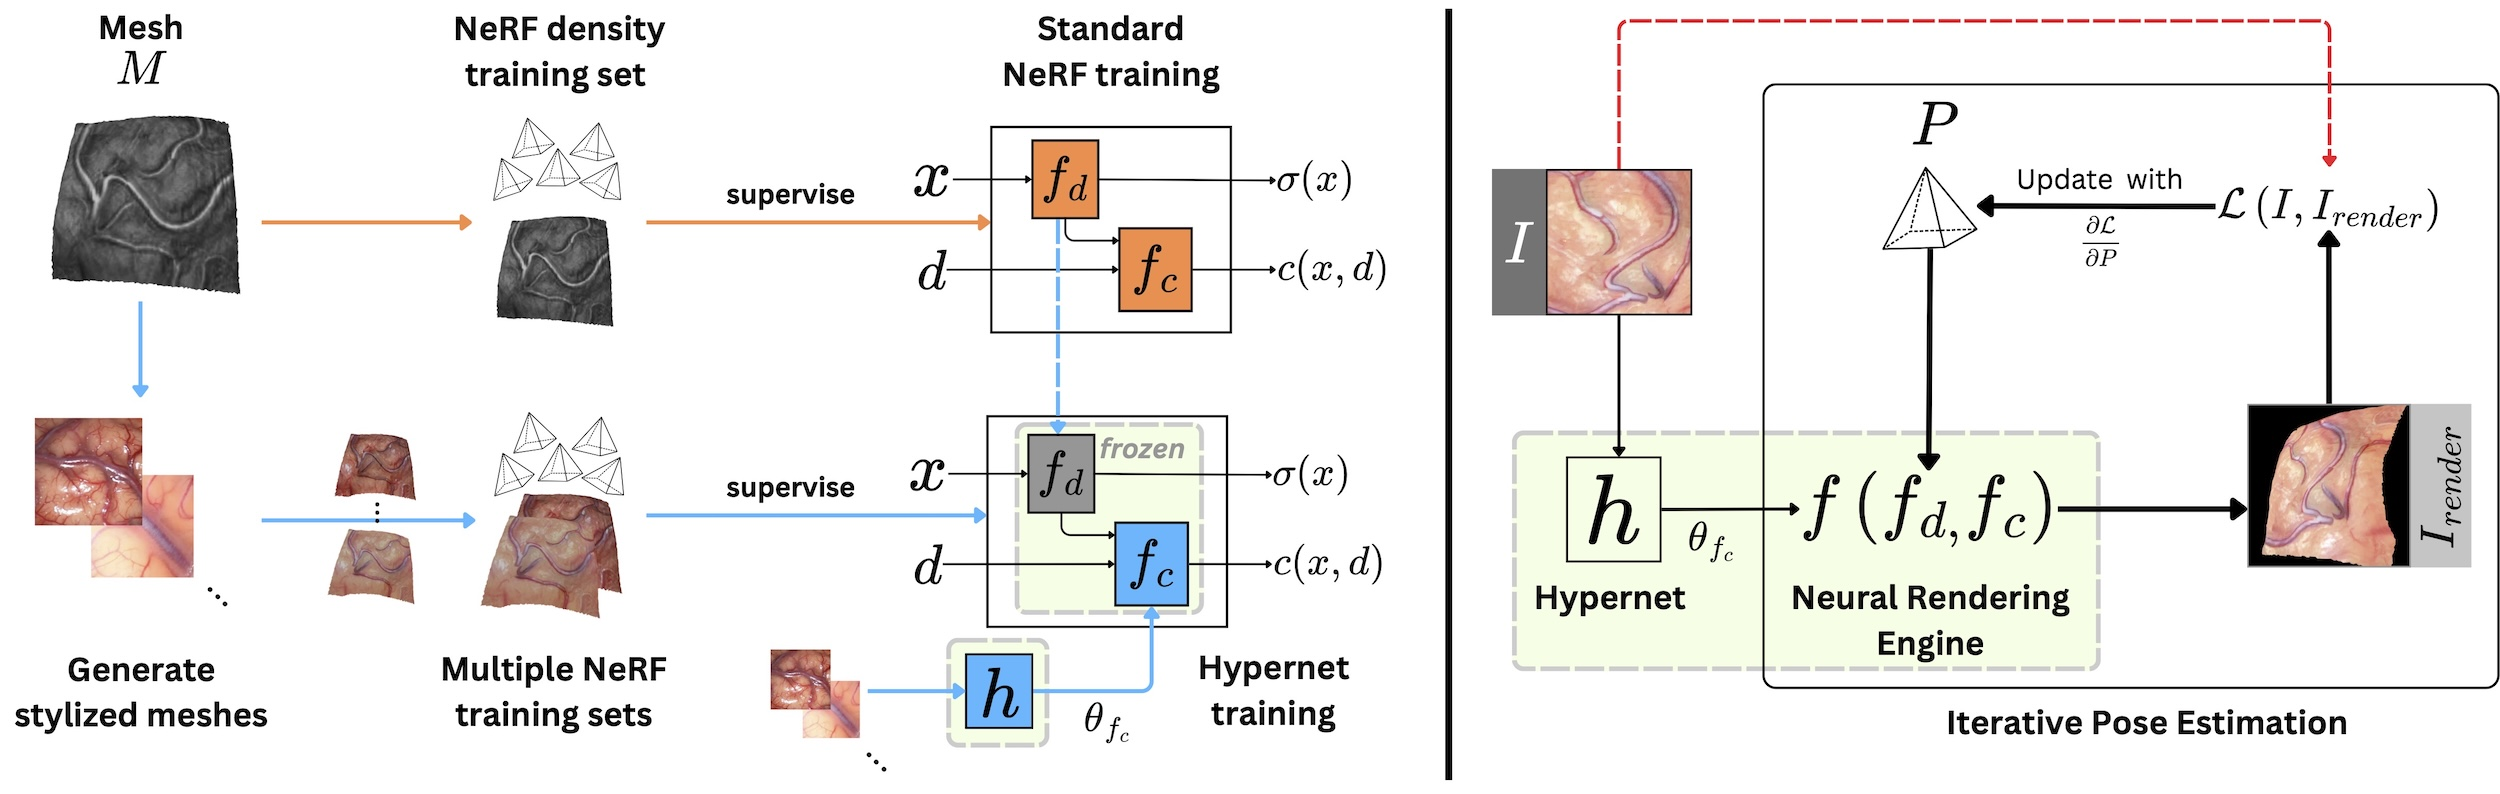
\includegraphics[width=0.9\textwidth]{figures/pipeline.jpg}
  \caption{Overview of the NeRF-based intraoperative registration approach. The method involves preoperative training of a NeRF model on MRI data, followed by intraoperative optimization of camera pose parameters to match the target surgical image.\parencite{fehrentz2024intraoperative}}
  \label{fig:overview}
\end{figure}

% add padding to the figure
\vspace{1cm}

The registration process consists of two main phases:

\begin{enumerate}
    \item \textbf{Preoperative Phase}: A NeRF model is trained using preoperative MRI data to create an implicit representation of the brain's structure.
    
    \item \textbf{Intraoperative Phase}: During surgery, the pre-trained NeRF is used as a differentiable rendering engine. Given a target intraoperative image, the camera pose (6 degrees of freedom) is optimized through a gradient-based approach to match the rendered view with the target image.
\end{enumerate}

\section{Implementation Framework}

One of the primary contributions of this thesis is the development of a flexible, model-agnostic implementation of neural registration built on the nerfstudio framework. Unlike previous implementations that were tied to specific NeRF variants, the proposed framework allows for seamless integration of different NeRF architectures and loss functions.

\subsection{Nerfstudio Integration}

The implementation leverages the nerfstudio framework to ensure flexibility and compatibility with various NeRF architectures. The key components include:

\begin{itemize}
    \item \textbf{Model Agnosticism}: The implementation works with multiple NeRF variants, including the original NeRF \parencite{mildenhall2020nerf}, Instant-NGP \parencite{muller2022instant}, and Nerfacto \parencite{Tancik_2023}, enabling evaluation of different architectures' impact on registration performance.
    
    \item \textbf{Registration Optimizer}: A dedicated optimizer module (the \texttt{iNeRFOptimizerBatchedFD} class) that handles camera pose optimization, loss computation, and experiment tracking.
    
    \item \textbf{Pluggable Loss Functions}: A modular interface for different loss functions, enabling systematic comparison of various similarity metrics.
\end{itemize}

The advantages of this implementation over previous approaches include:
\begin{itemize}
    \item Easy customization of loss functions without modifying the core registration algorithm
    \item Compatibility with nerfstudio's pre-trained models
    \item Integration capabilities with hypernetwork-based appearance adaptation
    \item Comprehensive experiment tracking and visualization
\end{itemize}

\subsection{Finite Difference Optimization}

A notable technical aspect of the implementation is the use of finite difference methods for gradient computation. During development, challenges were encountered with the gradient flow being disconnected in the computational graph when using standard backpropagation. To overcome this limitation while preserving the original concept, a batched finite difference approach for computing gradients was implemented:

\begin{algorithm}[H]
\caption{Batched Finite Difference Gradient Computation}
\begin{algorithmic}[1]
\State \textbf{Input:} Current pose parameters $\theta$, small perturbation $\epsilon$, batch size $B$
\State \textbf{Output:} Gradient $\nabla_{\theta} L$
\State $L_{\text{original}}, \_ \gets \text{ComputeLoss}(\theta)$ \Comment{Compute loss at current pose}
\State $\nabla_{\theta} L \gets \mathbf{0}$ \Comment{Initialize gradient}
\State $\text{coords} \gets \{(i,j) \text{ for all elements } \theta_{i,j} \text{ in } \theta\}$ \Comment{All parameter coordinates}
\For{batch\_start $= 0$ to $|\text{coords}|$ step $B$}
    \State batch\_coords $\gets \text{coords[batch\_start:batch\_start}+B]$
    \State batch\_poses $\gets [\:]$ \Comment{Initialize batch of perturbed poses}
    \For{$(i,j)$ in batch\_coords}
        \State $\theta' \gets \theta$
        \State $\theta'_{i,j} \gets \theta'_{i,j} + \epsilon$ \Comment{Perturb single parameter}
        \State Add $\theta'$ to batch\_poses
    \EndFor
    \State batch\_losses $\gets \text{ComputeBatchLosses(batch\_poses)}$
    \For{idx, $(i,j)$ in enumerate(batch\_coords)}
        \State $\nabla_{\theta_{i,j}} L \gets \frac{\text{batch\_losses[idx]} - L_{\text{original}}}{\epsilon}$ \Comment{Estimate gradient}
    \EndFor
\EndFor
\State \Return $\nabla_{\theta} L$
\end{algorithmic}
\end{algorithm}

This approach offers several advantages:
\begin{itemize}
    \item Robustness to disconnected gradients in the computational graph
    \item Efficient batch processing that significantly reduces computation time
    \item Compatibility with any NeRF model regardless of internal architecture
\end{itemize}

\section{Neural Registration Algorithm}

The complete neural registration algorithm using the implemented framework is presented below:

\begin{algorithm}[H]
\caption{NeRF-based Registration with Customizable Loss Functions}
\begin{algorithmic}[1]
\State \textbf{Input:} Pre-trained NeRF model $\mathcal{N}$, target image $I_{target}$, initial pose $\xi_0$, loss function $\mathcal{L}$, learning rate $\alpha$, number of iterations $T$
\State \textbf{Output:} Optimized camera pose $\hat{\xi}$
\State Initialize pose parameters $\xi \gets \xi_0$
\State Initialize optimizer with pose parameters and learning rate $\alpha$
\State best\_loss $\gets \infty$, best\_pose $\gets \xi_0$
\For{$t = 1$ to $T$}
    \State Compute gradient $\nabla_{\xi} \mathcal{L}$ using batched finite differences:
    \State \hspace{\algorithmicindent} $L_{original}, I_{rendered} \gets \text{ComputeLoss}(\xi)$ \Comment{Forward pass with current pose}
    \State \hspace{\algorithmicindent} $\nabla_{\xi} \mathcal{L} \gets \text{BatchedFiniteDifference}(\xi, L_{original})$
    \State Update pose parameters: $\xi \gets \xi - \alpha \cdot \nabla_{\xi} \mathcal{L}$ \Comment{Gradient descent step}
    \If{$L_{original} < \text{best\_loss}$}
        \State best\_loss $\gets L_{original}$
        \State best\_pose $\gets \xi$
    \EndIf
    \If{$t \bmod \text{visualize\_interval} = 0$}
        \State Visualize current alignment between $I_{target}$ and $I_{rendered}$
    \EndIf
\EndFor
\State \Return best\_pose
\end{algorithmic}
\end{algorithm}

The rendered image $I_{rendered}$ is generated by passing the current camera pose $\xi$ to the pre-trained NeRF model, which produces an RGB prediction. The loss $\mathcal{L}(I_{target}, I_{rendered})$ measures the dissimilarity between the target and rendered images using the selected loss function.

\subsection{Camera Pose Representation}

The camera pose is represented as a 3×4 transformation matrix with the following structure:
\begin{equation}
\xi = \begin{bmatrix} 
R_{11} & R_{12} & R_{13} & t_x \\
R_{21} & R_{22} & R_{23} & t_y \\
R_{31} & R_{32} & R_{33} & t_z
\end{bmatrix}
\end{equation}

where $R$ represents the 3×3 rotation matrix and $t$ represents the translation vector. This 3×4 matrix is converted to the appropriate camera representation using the nerfstudio Camera class during rendering.

\section{Loss Functions for NeRF-Based Registration}\label{section:loss_functions}


The effectiveness of NeRF-based registration fundamentally depends on the choice of loss function, which serves as the mathematical backbone guiding pose optimization. Loss functions quantify the dissimilarity between rendered and target images, effectively creating the optimization landscape that determines convergence behavior and registration accuracy. This section provides a comprehensive analysis of five distinct loss functions (L1, L2, Structural Similarity Index, Normalized Cross-Correlation, and Mutual Information) in the context of intraoperative neural registration. We examine their mathematical formulations, implementation considerations, and comparative performance to understand how different similarity metrics affect registration precision, convergence speed, and robustness to initialization variations. Our systematic evaluation reveals important insights into selecting appropriate loss functions for specific neural registration scenarios, particularly in neurosurgical applications where alignment accuracy directly impacts surgical outcomes.
\subsection{Role of Loss Functions in Registration}

In the context of intraoperative registration using Neural Radiance Fields, the loss function serves two primary purposes:

\begin{enumerate}
    \item \textbf{Similarity Measurement}: It quantifies the similarity between the target intraoperative image and the rendered image from the NeRF model, guiding the optimization process toward better alignment.
    
    \item \textbf{Gradient Provision}: It provides gradients with respect to camera pose parameters, enabling optimization of the camera pose.
\end{enumerate}

\subsection{Implemented Loss Functions}

This section details the loss functions implemented and evaluated in this thesis. Further implementation details can be found in Appendix~\ref{appendix:implementation}. 

\subsubsection{L1 Loss}

The L1 loss, or mean absolute error, calculates the absolute difference between pixel values:

\begin{equation}
\mathcal{L}_{L1}(I_1, I_2) = \frac{1}{N} \sum_{i=1}^{N} |I_1(i) - I_2(i)|
\end{equation}

where $N$ is the number of pixels in the images.

Key characteristics of L1 loss include:
\begin{itemize}
    \item Less sensitivity to outliers compared to L2 loss
    \item Linear behavior that can lead to faster convergence in some cases
    \item Simple gradients that are constant with respect to the error magnitude
\end{itemize}

\subsubsection{L2 Loss}

The L2 loss, or mean squared error (MSE), is the standard baseline approach:

\begin{equation}
\mathcal{L}_{L2}(I_1, I_2) = \frac{1}{N} \sum_{i=1}^{N} (I_1(i) - I_2(i))^2
\end{equation}

Key characteristics of L2 loss include:
\begin{itemize}
    \item Quadratic penalization of large errors
    \item Gradients that scale with the magnitude of the error
    \item Sensitivity to outliers
\end{itemize}

\subsubsection{Structural Similarity Index Loss}

The Structural Similarity Index Measure (SSIM) captures structural information in images:

\begin{equation}
\text{SSIM}(x, y) = \frac{(2\mu_x\mu_y + C_1)(2\sigma_{xy} + C_2)}{(\mu_x^2 + \mu_y^2 + C_1)(\sigma_x^2 + \sigma_y^2 + C_2)}
\end{equation}

The SSIM loss is then defined as:
\begin{equation}
\mathcal{L}_{\text{SSIM}}(I_1, I_2) = 1 - \text{SSIM}(I_1, I_2)
\end{equation}

Key characteristics of SSIM loss include:
\begin{itemize}
    \item Focus on structural information rather than pixel-wise differences
    \item Invariance to certain local transformations
    \item Better correlation with human visual perception
\end{itemize}

\subsubsection{Normalized Cross-Correlation (NCC)}

Normalized Cross-Correlation measures the linear relationship between two images while being invariant to linear intensity transformations:

\begin{equation}
\text{NCC}(I_1, I_2) = \frac{\sum_{i=1}^{N} (I_1(i) - \bar{I}_1)(I_2(i) - \bar{I}_2)}{\sqrt{\sum_{i=1}^{N} (I_1(i) - \bar{I}_1)^2 \sum_{i=1}^{N} (I_2(i) - \bar{I}_2)^2}}
\end{equation}

The NCC loss is then defined as:
\begin{equation}
\mathcal{L}_{\text{NCC}}(I_1, I_2) = 1 - \text{NCC}(I_1, I_2)
\end{equation}

Key characteristics of NCC loss include:
\begin{itemize}
    \item Invariance to linear intensity transformations
    \item Robustness to global illumination changes
    \item Effectiveness for cross-modal registration tasks
\end{itemize}

\subsubsection{Mutual Information (MI)}

Mutual Information quantifies the statistical dependence between two random variables:

\begin{equation}
\text{MI}(I_1, I_2) = \sum_{i,j} p_{I_1,I_2}(i,j) \log\left(\frac{p_{I_1,I_2}(i,j)}{p_{I_1}(i)p_{I_2}(j)}\right)
\end{equation}

The MI loss is defined as:
\begin{equation}
\mathcal{L}_{\text{MI}}(I_1, I_2) = -\text{MI}(I_1, I_2)
\end{equation}

Key characteristics of MI loss include:
\begin{itemize}
    \item Ability to capture complex, non-linear relationships between image intensities
    \item Suitability for cross-modal registration
    \item Robustness to partial overlap between images
\end{itemize}

\section{Experimental Setup}

To rigorously evaluate the impact of different loss functions on Neural Radiance Field (NeRF) based intraoperative registration, a systematic experimental framework was designed with controlled variables and precise measurement protocols.

\subsection{Technical Configuration}

The experiments were conducted with the following specifications to ensure fair and consistent comparison across loss functions:
\begin{itemize}
    \item \textbf{Optimization Parameters}: Fixed at 50 iterations across all experiments to standardize convergence conditions
    \item \textbf{Optimization Algorithm}: AdamW optimizer with a learning rate of 0.01, chosen for its adaptive momentum properties and weight decay regularization
    \item \textbf{Gradient Computation}: Finite difference approximation with epsilon value of $1 \times 10^{-4}$ for gradient stability
    \item \textbf{Experimental Runs}: 10 different initial camera poses per loss function to ensure statistical significance and account for local optimization challenges
    \item \textbf{Target Consistency}: Identical target image used across all experiments to eliminate target-specific biases
    \item \textbf{Data Source Control}: Both target images and rendered views sourced from the same pre-trained NeRF model to eliminate variations due to domain gaps or rendering inconsistencies
    \item \textbf{Batch Size}: Set at 12 for finite difference calculations to optimize the trade-off between memory usage and computational efficiency
\end{itemize}

\subsection{Loss Functions}

As previously introduced in Section~\ref{section:loss_functions}, five distinct loss functions were systematically evaluated to compare their performance in NeRF-based registration:

\begin{itemize}
    \item \textbf{L1 Loss (Mean Absolute Error)}
    
    \item \textbf{L2 Loss (Mean Squared Error)}
    
    \item \textbf{Structural Similarity Index Loss (SSIM)}
    
    \item \textbf{Normalized Cross-Correlation (NCC)}
    
    \item \textbf{Mutual Information Loss (MI)}
\end{itemize}

Each loss function was selected for its unique properties and potential advantages in medical image registration: L1 and L2 for their direct intensity comparisons with different sensitivity to outliers; SSIM for its emphasis on structural information; NCC for its robustness to linear intensity variations; and MI for its capacity to handle multi-modal image alignment.

\subsection{Evaluation Metrics}

Registration performance was comprehensively evaluated using the following quantitative and qualitative metrics:

\begin{itemize}
    \item \textbf{Convergence Efficiency}: Measured by identifying the iteration at which the optimal loss value was achieved, providing insight into each loss function's optimization trajectory
    
    \item \textbf{Computational Performance}: Total time required for the complete optimization process, broken down into component stages including forward passes, gradient calculations, and parameter updates
    
    \item \textbf{Registration Accuracy}: Quantified through:
    \begin{itemize}
        \item Final loss value achieved
        \item Pixel-wise alignment between registered and target images
        \item Visual overlay assessment by superimposing the registered image on the target with 50\% transparency
    \end{itemize}
    
    \item \textbf{Optimization Stability}: Analyzed through:
    \begin{itemize}
        \item Loss curve smoothness and monotonicity
        \item Variance in pose parameter updates across iterations
        \item Resistance to local minima in the optimization landscape
    \end{itemize}
    
    \item \textbf{Robustness to NeRF Artifacts}: Qualitative assessment of how each loss function performs in the presence of rendering inconsistencies
\end{itemize}

\subsection{Experiment Tracking and Data Collection}

A comprehensive tracking framework was implemented to capture all relevant experimental data:

\begin{itemize}
    \item \textbf{Parameter Trajectory}: Complete camera pose transformation matrix recorded at each iteration
    
    \item \textbf{Loss Dynamics}: Full loss history with values captured after each optimization step
    
    \item \textbf{Visual Documentation}: 
    \begin{itemize}
        \item Rendered images saved at regular intervals (every 10 iterations)
        \item Side-by-side visualizations of target and current rendered images
        \item Progressive alignment overlays to visually track registration improvement
    \end{itemize}
    
    \item \textbf{Performance Profiling}:
    \begin{itemize}
        \item Per-iteration timing statistics
        \item Computational resource utilization
        \item Batch processing efficiency metrics for finite difference calculations
    \end{itemize}
    
    \item \textbf{Metadata Management}: Structured JSON tracking files containing complete experimental parameters, iteration history, and final results for reproducibility and further analysis
\end{itemize}

All experimental data was systematically organized in a standardized directory structure to facilitate comparative analysis and ensure reproducibility of results.

\section{Summary}

This chapter has presented a comprehensive methodology for enhancing intraoperative registration using Neural Radiance Fields. The key contributions include:

\begin{enumerate}
    \item Development of a flexible, model-agnostic implementation of neural registration integrated with the nerfstudio framework
    \item Implementation of a batched finite difference approach for robust gradient computation
    \item Systematic evaluation of multiple loss functions (L1, L2, SSIM, NCC, MI) for NeRF-based registration
    \item A controlled experimental setup for fair comparison of different approaches
\end{enumerate}

The results of these experiments are presented and analyzed in Chapter~\ref{chapter:results}. 